% Dokumentklassen:
% article, report, beamer, book, letter etc.
% https://en.wikibooks.org/wiki/LaTeX/Document_Structure
\documentclass[a4paper]{article}

% Seitenränder Abstand setzen
\usepackage[margin=80pt]{geometry}

% Deutsches Sprachpaket
\usepackage[ngerman]{babel}
% UTF8 Input Encoding
\usepackage[utf8]{inputenc}

% Schriftbild ändern
% https://en.wikibooks.org/wiki/LaTeX/Fonts
\usepackage[scaled]{helvet}
% (Sans) Serifen oder anderes
% \rmdefault: Serifen
% \sfdefault: Sans-Serifen
% \ttdefault: Typewriter
\renewcommand{\familydefault}{\sfdefault}
% Fontencoding (für ä, ö, ü etc.)
\usepackage[T1]{fontenc}

% Gänsefüsschen richtig kompilieren
\usepackage [autostyle]{csquotes}
\MakeOuterQuote{"}

% Hyperlinks farblos
\usepackage[hidelinks]{hyperref}
\hypersetup{colorlinks=false}

% Package für Aufzählungen
\usepackage{enumitem}
% kein Abstand zwischen Aufzählungen
% Sollen doch Abstände vorhanden sein: nach Aufzählung {itemsep=1em}
\setlist{nosep}

% Grafik-Packages, für Figures, Subfigures und PDF als Import
\usepackage{graphicx}
\usepackage{subcaption}
\usepackage{pdfpages}

% Package und Einstellungen für Java-Code-Darstellung
% Werden erstellt mit \begin{lstlisting}
\usepackage{listings}
\usepackage{color}
\definecolor{dkgreen}{rgb}{0,0.6,0}
\definecolor{gray}{rgb}{0.5,0.5,0.5}
\definecolor{mauve}{rgb}{0.58,0,0.82}
\lstset{frame=tb,
	language=Java,
	aboveskip=3mm,
	belowskip=3mm,
	showstringspaces=false,
	columns=flexible,
	basicstyle={\small\ttfamily},
	numbers=none,
	numberstyle=\tiny\color{gray},
	keywordstyle=\color{blue},
	commentstyle=\color{dkgreen},
	stringstyle=\color{mauve},
	breaklines=true,
	breakatwhitespace=true,
	tabsize=3
}

\title{\textbf{Zusammenfassung DL4G} \\
		Deep Learning for Games}
\date{\today}
\author{Maurin D. Thalmann}

\begin{document}
	
	\pagenumbering{gobble}
	\maketitle
	
	\newpage
	\pagenumbering{arabic}
	\tableofcontents
	
	\newpage
	
	\section{Sequential Games with perfect information}
	
		\subsection{Finite Sequential Games}
		
		\begin{itemize}
			\item Eine endliches Set an \textbf{Spielern}, jeder mit einem endlichen Set an möglichen \textbf{Aktionen}
			\item Spieler wählen ihre Aktionen \textbf{sequenziell} (einer nach dem anderen, in Zügen)
			\item Eine endliche Anzahl an \textbf{Zügen} wird gespielt
			\item Spätere Spieler \textbf{beobachten} die Züge der früheren Spieler (Perfect Recall)
			\item Eine \textbf{Strategie} sagt dem Spieler, welche Aktion er in seinem Zug spielen soll
			\item Ein \textbf{Strategieprofil} ist eine gewählte Strategie eines jeden Spielers
			\item Ein \textbf{Utility} oder \textbf{Payoff Function} bestimmt den Ausgang jedes Aktionprofils
		\end{itemize}
	
		\subsection{Complexity Factors in Game Analysis}
		
		\begin{enumerate}
			\item Anzahl Spieler
			\begin{itemize}
				\item Spiele mit 4 Spielern sind schwieriger zu analysieren als solche mit 2 Spielern
			\end{itemize}
			\item Grösse des Suchraums
			\begin{itemize}
				\item Bestimmt durch Anzahl gespielte Züge und Anzahl Aktionen für jeden Spieler
			\end{itemize}
			\item Kompetitive Spiele vs. Kooperative Spiele
			\begin{itemize}
				\item Kompetitive Spiele involvieren Spieler mit komplett gegensätzlichen Interessen 
			\end{itemize}
			\item Stochastische Spiele vs. Deterministische Spiele
			\begin{itemize}
				\item Stochastische Spiele beinhalten Zufälle, bspw. Verteilung der Karten, Würfel rollen
			\end{itemize}
			\item Perfekte vs. imperfekte Informationsspiele
			\begin{itemize}
				\item Imperfekte Information heisst das Spiel ist nur teilweise überwachbar, bspw. kennen wir nicht die Karten eines gegnerischen Spielers beim Poker oder Jass
			\end{itemize}
		\end{enumerate}
	
		\subsection{Illustration of State Space Complexity}
		
		\begin{table}[htb!]
			\begin{tabular}{ |c|c|}
				\textbf{Game} & \textbf{\begin{tabular}[c]{@{}c@{}}State Space\\ (as log to base 10; 10$^x$)\end{tabular}} \\
				Tic-Tac-Toe   & 3                                                                                                         \\
				Connect-4     & 13                                                                                                        \\
				Backgammon    & 20                                                                                                        \\
				Chess         & 47                                                                                                        \\
				Go 19x19      & 170                                                                                                      
			\end{tabular}
		\end{table}
	
		\begin{itemize}
			\item State Space beschreibt die Anzahl erlaubter Boardpositionen
			\item Schach / Chess hat 10$^{47}$ verschiedene Boards, Go hat 10$^{170}$ verschiedene Boards
			\item Zum Vergleich: Geschätzt sind im Universum 10$^{80}$ Atome
		\end{itemize}
	
		\subsection{Extensive Form Representation}
	
		\begin{itemize}
			\item Sequenzielle Spiele können (im Prinzip) als Spielbäume repräsentiert werden
			\item Knoten sind Spielzustände/Positionen und Kanten sind Aktionen/Bewegungen
			\item Blätter (Leaves) bestimmen den Payoff
		\end{itemize}
	
		\newpage
	
		\subsection{Game Tree Analysis - Backward Induction}
		
		\begin{figure}[htb!]
			\centering
			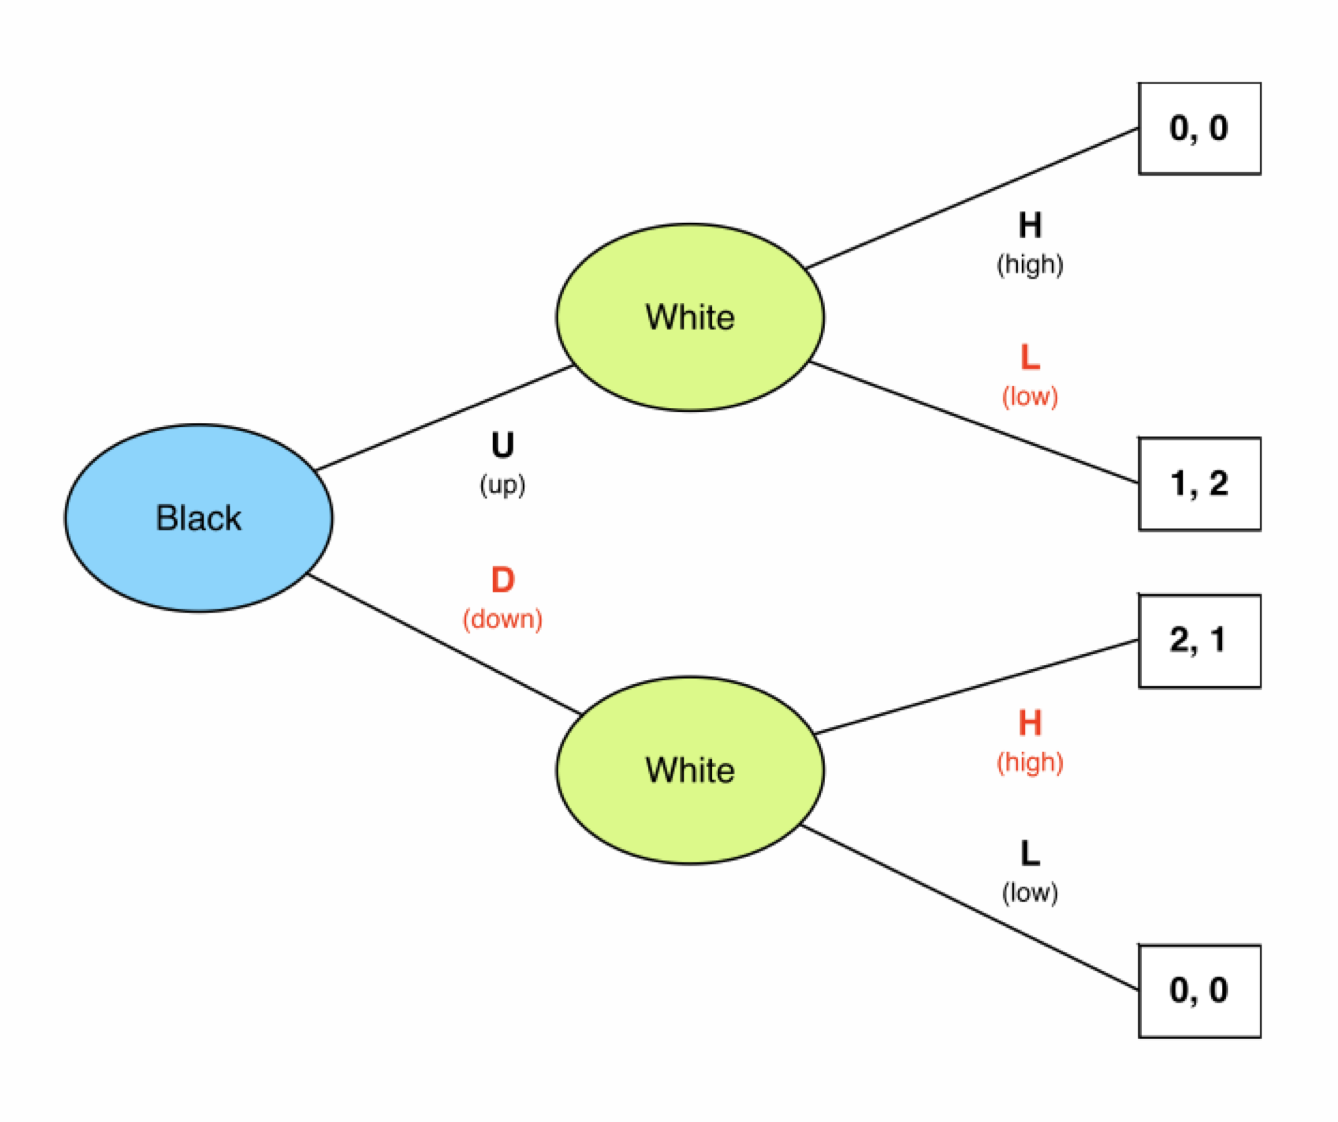
\includegraphics[width=0.6\textwidth]{img/01_sequential_games/gametree_backward_induction.png}
			\caption{Backward Induction am Beispiel eines simplen Spielbaums}
			\label{fig:01_seq_backward_induction}
		\end{figure}
	
		\begin{itemize}
			\item Backward Induction ist der Lösungsalgorithmus für endliche, sequenzielle Spiele
			\item Im Beispiel oben hat Black den First-Mover Vorteil.
			\item Wenn beide Spieler perfekt spielen, endet das Spiel mit den Payoffs (2,1) \\
				(2 für Black, 1 für White)
			\item Solche Spiele immer rückwärts analysieren!
		\end{itemize}
	
		\subsection{Reasoning about Finite Sequential Games}
		
		\begin{itemize}
			\item Eine \textbf{ultra-schwache Lösung} beweist ob der erste Spieler aus der Initialposition gewinnen, verlieren oder unentschieden machen wir, in Annahme eines perfekten Spiels des Gegners \\
			\textit{Im Beispiel: Schwarz kann einen Gewinn forcieren und hat demnach den First-Mover Vorteil}
			
			\item Eine \textbf{schwache Lösung} bietet einen Algorithmus welcher ein komplettes Spiel an perfekten Zügen aus der Initialposition offenbart, in Annahme eines perfekten Spiels des Gegners \\
			\textit{Schwache Lösung für das Spiel: Black spielt U, White spielt L, Black spielt D}
			
			\item Eine \textbf{starke Lösung} bietet einen Algorithmus, welcher perfekte Züge aus jeder Position produzieren kann, auch wenn vorher von irgendeinem Spieler Fehler gemacht wurden. \\
			\textit{Starke Lösung für dieses Spiel:}
				\begin{itemize}
					\item \textit{Algorithmus für White: wenn Black U spielt $\rightarrow$ spiel L; wenn Black D spielt $\rightarrow$ spiel H}
					\item \textit{Algorithmus für Black: Spiel D im ersten Zug; wenn White L im oberen Knoten spielt, spiel D}
				\end{itemize}
		\end{itemize}
	
		\paragraph{A Strong Solution to Nim}
		
		Algorithmus für einen perfekten Nim Bot:
		
		\begin{enumerate}
			\item Wenn nur ein Haufen übrig bleibt \\
				$\rightarrow$ Nimm alle Objekte des Haufens und hol den Preis
			\item Wenn zwei Haufen mit unterschiedlicher Anzahl Objekte übrig bleiben \\
				$\rightarrow$ Nimm Objekte vom grösseren Haufen und mache beide gleich gross
			\item Wenn zwei Haufen diesselbe Anzahl Objekte haben \\
				$\rightarrow$ Egal was du tust, du hast verloren (in Annahme eines perfekten Spiels des Gegners)
		\end{enumerate} 
	
		\newpage
	
		\subsection{Zero-Sum Games}
		
		\begin{itemize}
			\item Ein Spiel ist Zero-Sum, wenn der totale Gewinn des Siegers gleich dem totalen Verlust des Verlierers ist
				\begin{itemize}
					\item Einen Kuchen zu schneiden ist zero-sum bspw. wenn ich ein Stück esse, ist es für dich verloren
					\item Brettspiele sind zero-sum bspw. wenn der Sieger +1 erhält und der Verlierer -1
				\end{itemize}
			\item $u_{1}$ und $u_{2}$ umschreiben die Utility-Funktion von Spieler 1 und 2, somit ist für jedes Strategiepaar $s_{1}$ und $s_{2}$ von Spieler 1 und 2 und es gilt $u_{1}(s_{1}, s_{2}) + u_{2}(s_{1}, s_{2}) = 0$, dann lässt sich sagen: \\
			$$u_{1}(s_{1}, s_{2}) = -u_{2}(s_{1}, s_{2})$$
		\end{itemize}
	
		\paragraph{Backward Induction \& Minimax}
		
		\begin{itemize}
			\item Backward Induction ist die Lösungsstrategie für endliche Spiele mit perfekter Information
			\item Eine einzelne Durchführung von Backward Induction aus einem Startzustand offenbart eine schwache Lösung.
			Wenn Backward Induction dynamisch (während des Spiels) aus jedem Zustand ausgeführt werden kann, erhalten wir eine starke Lösung.
			\item Wenn das Spiel zusätzlich zero-sum ist, kann Backward Induction mit dem Minimax Algorithmus implementiert werden.
			Minimax wird oft für Zwei-Spieler-Spiele definiert, ist aber auch für mehr Spieler erweiterbar.
			\item Minimax erlaubt effizientes Pruning ("Ausästen") und nahtlose Integration von Heuristiken
			\item Hinweis: Backward Induction kann auch für Spiele genutzt werden, die nicht zero-sum sind und kompliziertere Payoffs enthalten als eine einzelne Zahl
		\end{itemize}
	
		\subsection{Minimax Algorithm}
		
		\begin{itemize}
			\item 1928 von John von Neumann erfunden
			\item Beide Spieler wollen ihre respektiven Payoffs maximieren
			\item Weil das Spiel zero-sum ist, ist mein Gewinn = Verlust des Gegners
			\item Anstatt nach eigenem Gewinn zu maximieren, kann der Gewinn des Gegeners minimiert werden
			\item Im Spielbaum kann folgendermassen vorgegangen werden:
				\begin{itemize}
					\item Gehört der Knoten mir, wähle die Aktion welche den Payoff maximiert
					\item Gehört der Knoten dem Gegner, wähle die Aktion welche den Payoff minimiert
				\end{itemize}
		\end{itemize}
	
		\begin{figure}[htb!]
			\centering
			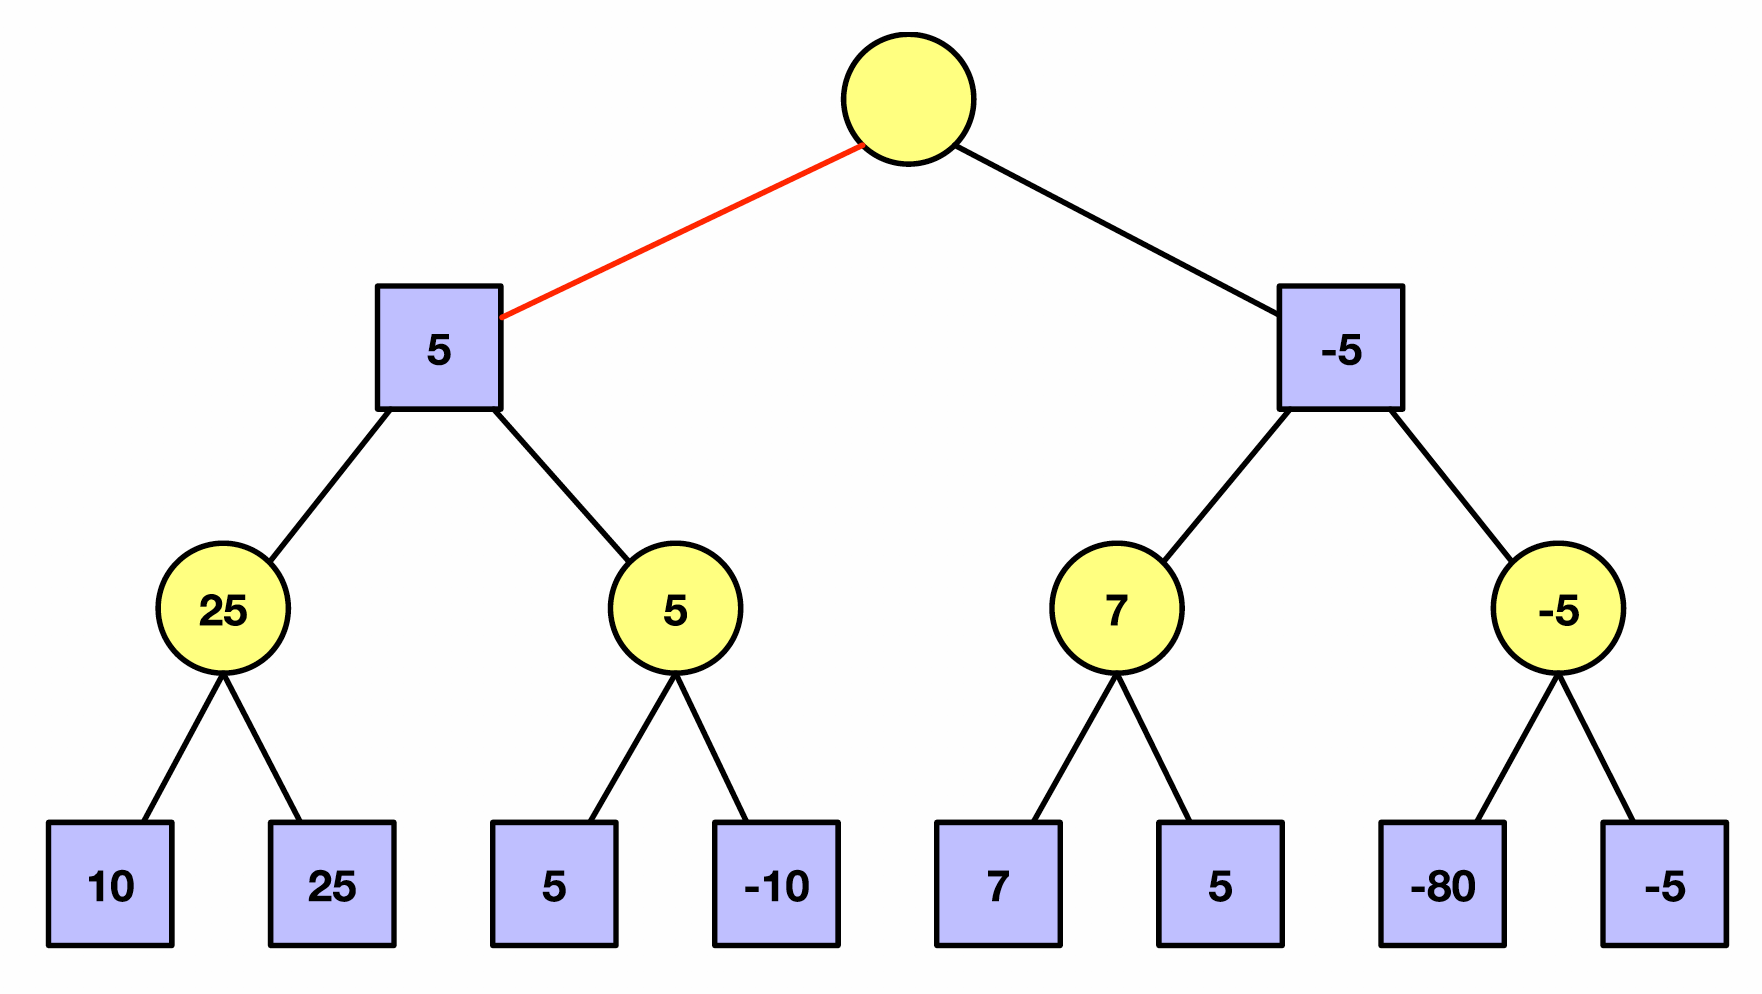
\includegraphics[width=0.6\textwidth]{img/01_sequential_games/minimax_solution.png}
			\caption{Lösungsweg eines Spielbaums mithilfe des Minimax-Algorithmus}
			\label{fig:01_seq_minimax_solution}
		\end{figure}
	
		\paragraph{Programming a Minimax Bot}
		
		\begin{itemize}
			\item Minimax implementiert Backward Induction für zero-sum Spiele.
				Dank der vereinfachenden zero-sum Eigenschaft können einige Tricks angewandt werden, um einen herusitischen Algorithmus zu erhalten:
			\begin{itemize}
				\item Minimax nur bis zu einer limitierten Tiefe, bspw. 5 Runden vorausschauen und dann stoppen.
					Wie tief man gehen kann ist abhängig von den Spielregeln (Anzahl mögliche Züge), Effizienz der Implementation und Rechenleistung.
				\item Da die Tiefe limitiert ist, werden die Blattknoten nicht erreicht und wir kennen die echten Payoffs nicht.
					Wir müssen eine Heuristik erfinden, um die Situation abzuschätzen an welcher wir stoppen.
					Je besser die Heuristik, desto besser der Bot.
			\end{itemize}
		\end{itemize}
	
		\begin{figure}[htb!]
			\centering
			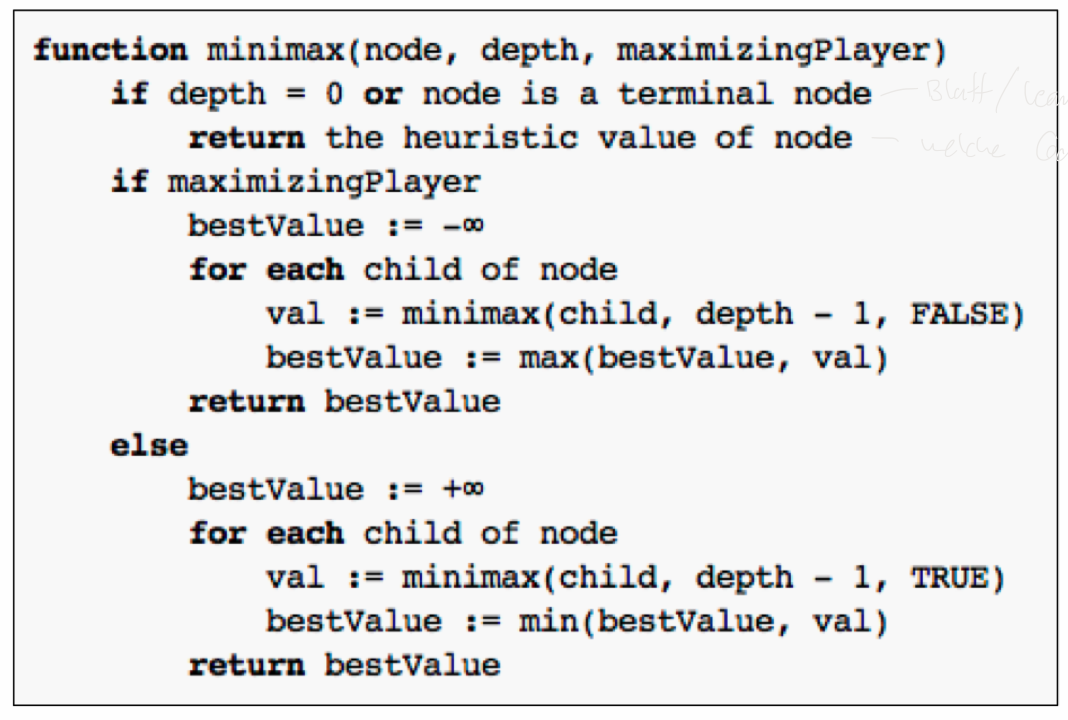
\includegraphics[width=0.6\textwidth]{img/01_sequential_games/minimax_pseudocode.png}
			\caption{Pseudocode eines Minimax-Algorithmus mit limitierter Tiefe und Heuristik}
			\label{fig:01_seq_minimax_pseudocode}
		\end{figure}
	
		\subsection{Search Tree Pruning}
		
		\begin{itemize}
			\item Es müssen nicht alle Knoten abgelaufen werden, um die optimale Strategie zu finden.
			\item Wir "stutzen" (prunen) Sub-Bäume, welche keine bessere Lösung beinhalten können und demnach nicht besucht werden müssen.
			\item Dazu enthält der Algorithmus zwei Parameter: \\
			\textit{(Vorfahren sind alle Knoten auf dem Weg zwischen dem aktuellen und dem Wurzelknoten)}
				\begin{itemize}
					\item $\alpha$ ist der höchste Wert aller MAX-Vorfahren eines MIN Knoten
					\item $\beta$ ist der tiefste Wert alles MIN-Vorfahren eines MAX Knoten
				\end{itemize}
			\item Der Algorithmus Alpha-Beta Pruning aktualisiert diese beiden Parameter im Minimax-Prozess und schneidet nicht besuchte Sub-Bäume ab, sobald er weiss dass die Werte aus diesem Sub-Baum den Wert $\alpha$ nicht überbieten oder $\beta$ nicht unterbieten können.
		\end{itemize}
		
		\paragraph{Alpha-Beta Pruning Rules}
		
		\begin{itemize}
			\item Alpha ($\alpha$) ist der minimale Score, welcher dem maximierenden Spieler versichert werden kann
			\item Beta ($\beta$) ist der maximale Score, welcher dem minimierenden Spieler versichert werden kann
			\item Daraus lassen sich folgende beiden Regeln schliessen:
				\begin{itemize}
					\item \textbf{Regel 1}: Schneide ab, sobald der aktuelle Wert eines MIN Knoten kleiner ist als $\alpha$
					\item \textbf{Regel 2}: Schneide ab, sobald der aktuelle Wert eines MAX Knoten grösser ist als $\beta$
				\end{itemize}
		\end{itemize}
	
		\subsection{Illustrations for Alpha-Beta Pruning}
		
		\begin{figure}[htb!]
			\centering
			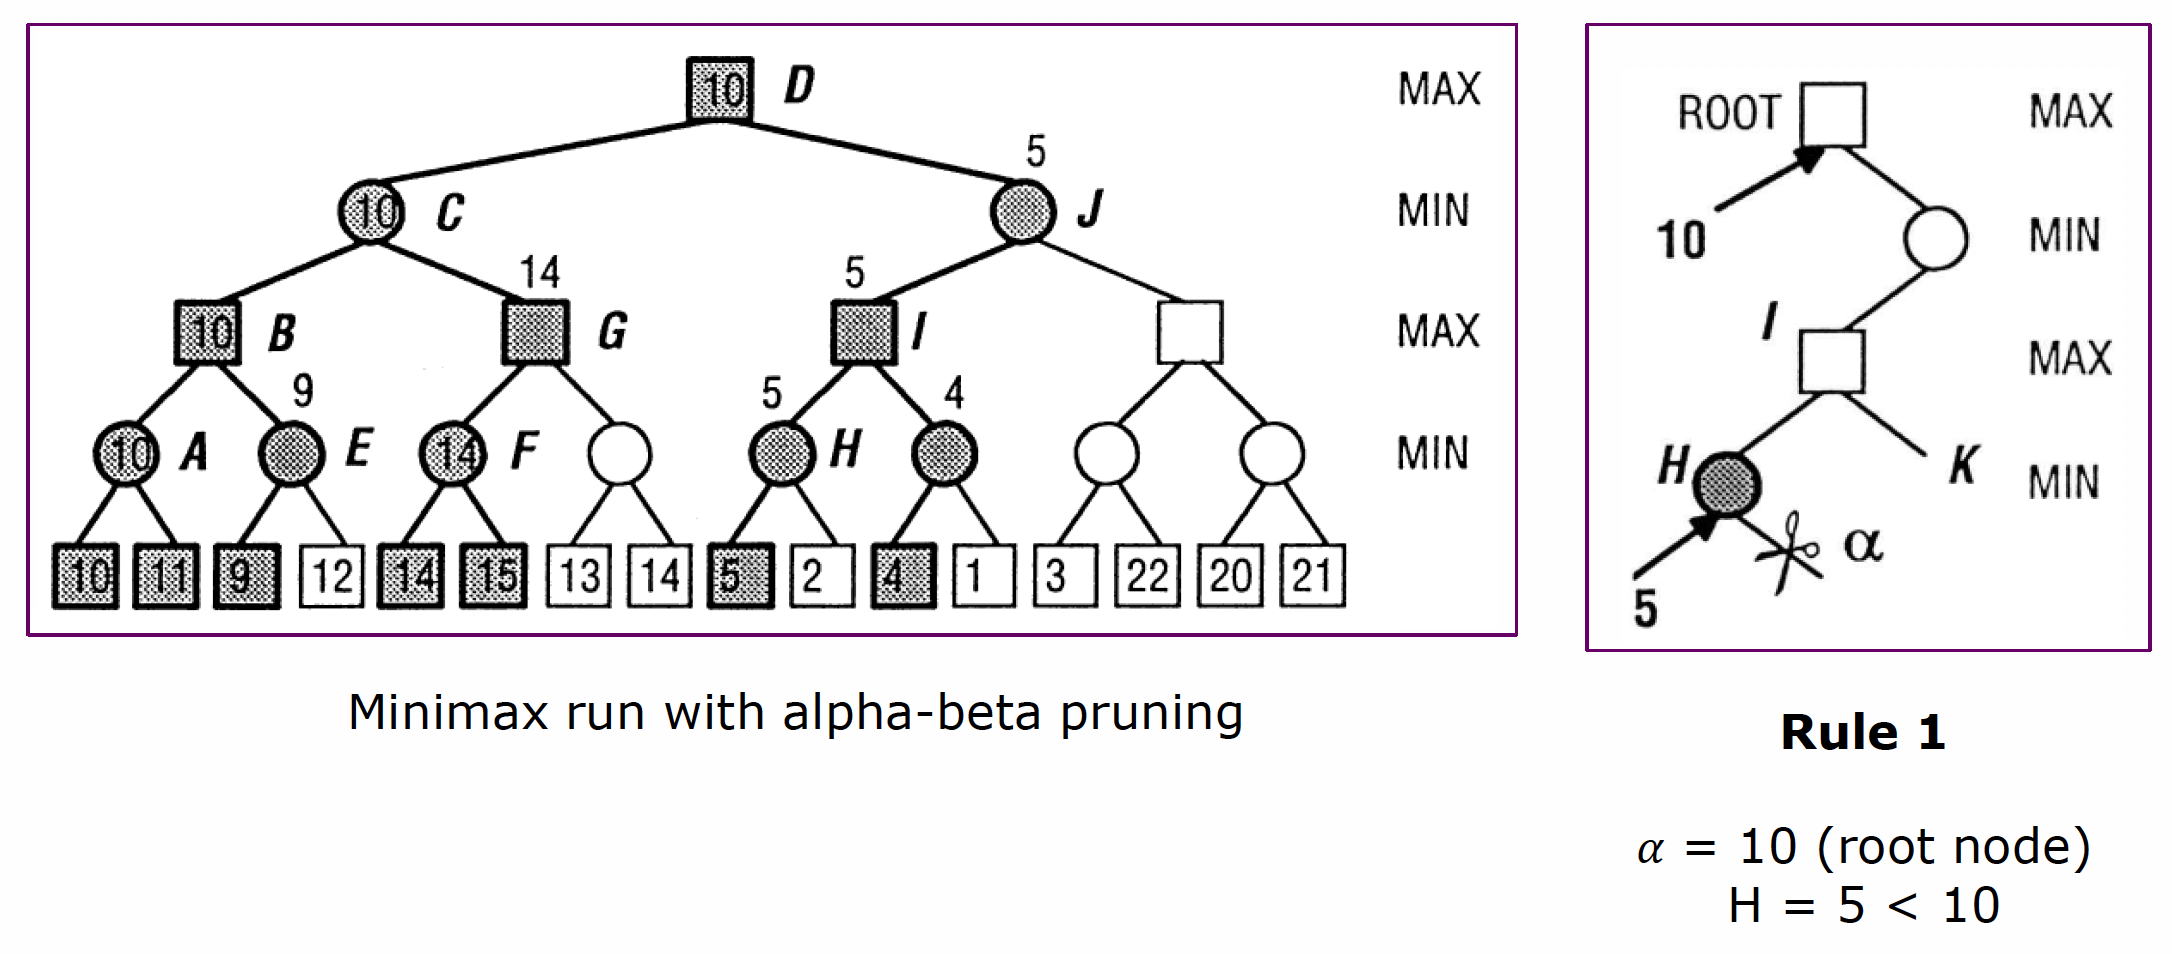
\includegraphics[width=0.5\textwidth]{img/01_sequential_games/alphabeta_rule1.png}
			\caption{Illustration der Durchführung der 1. Regel des Alpha-Beta Pruning}
			\label{fig:01_seq_alphabeta_rule1}
		\end{figure}
	
		\begin{figure}[htb!]
			\centering
			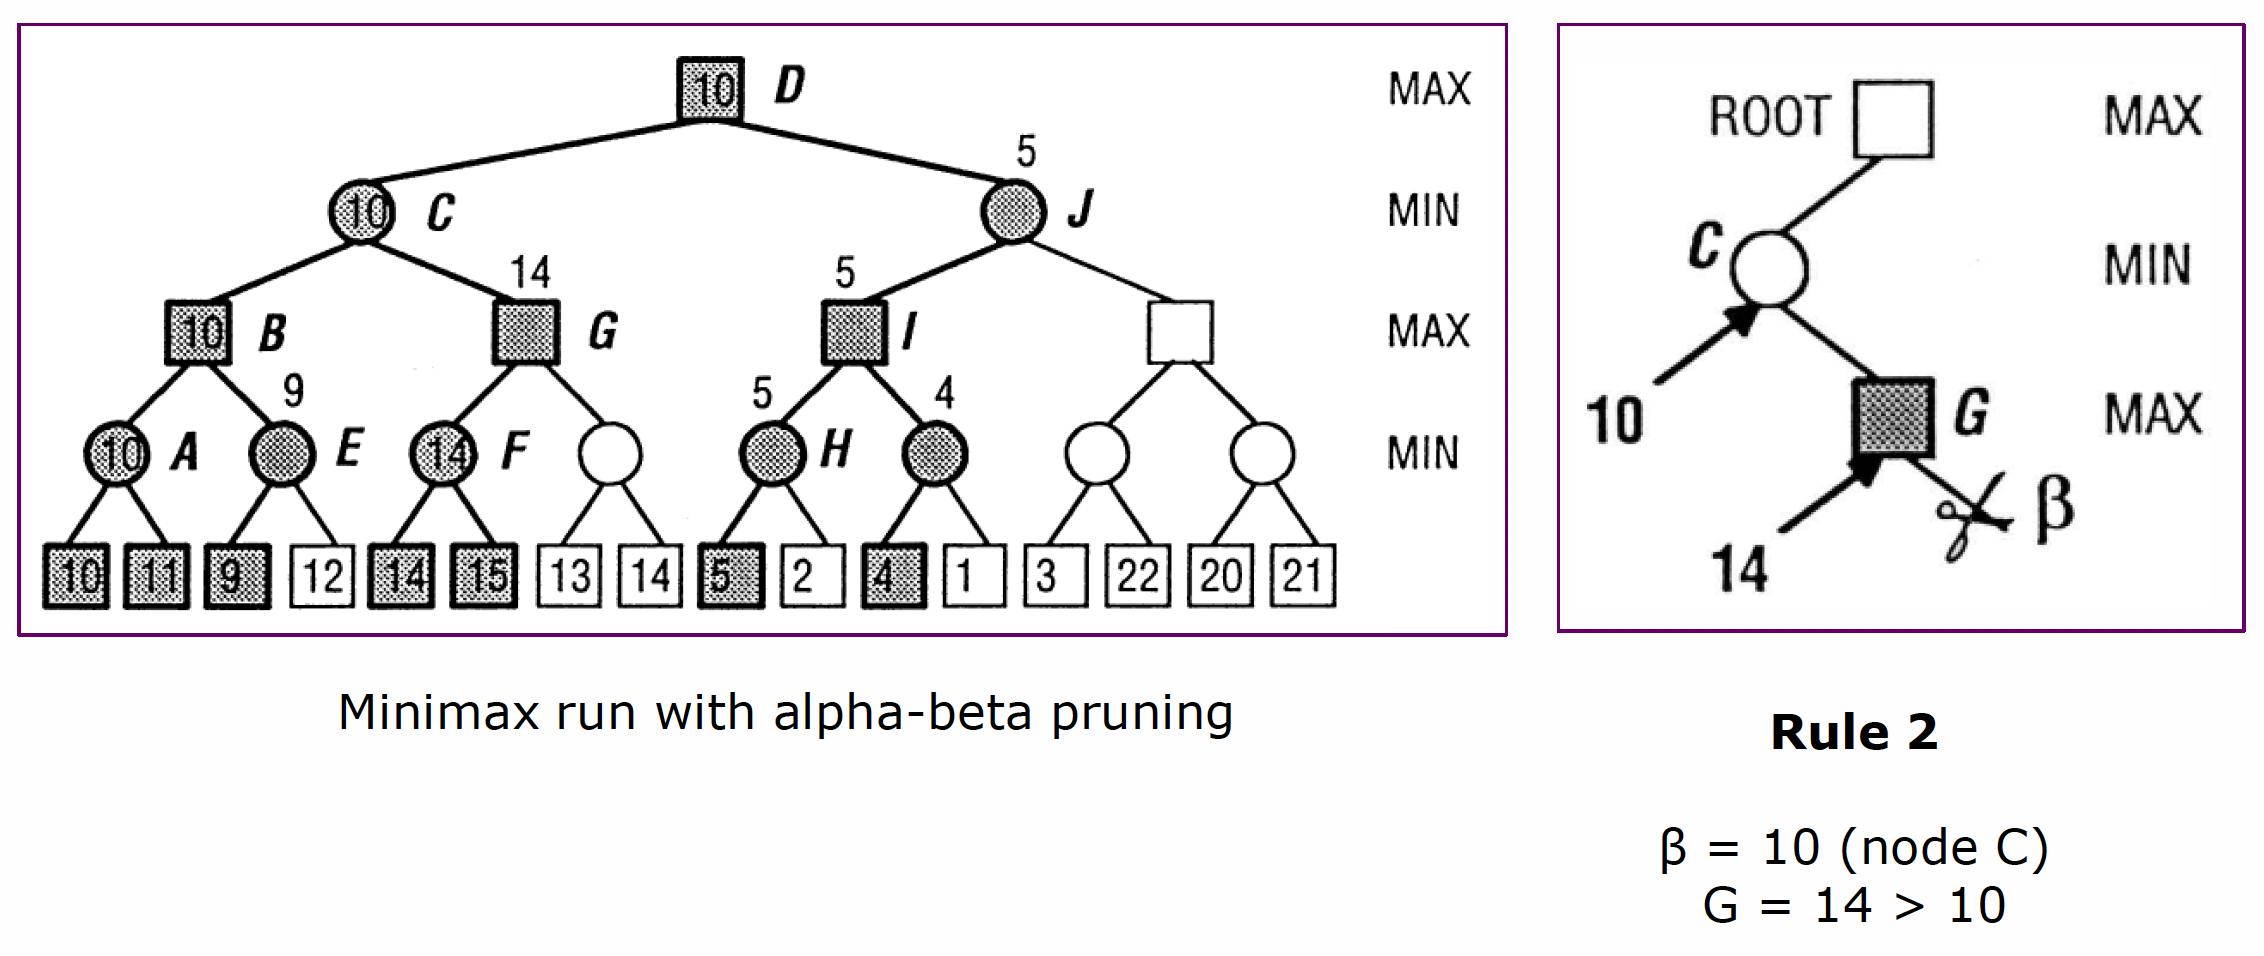
\includegraphics[width=0.5\textwidth]{img/01_sequential_games/alphabeta_rule2.png}
			\caption{Illustration der Durchführung der 2. Regel des Alpha-Beta Pruning}
			\label{fig:01_seq_alphabeta_rule2}
		\end{figure}
	
		\begin{figure}[htb!]
			\centering
			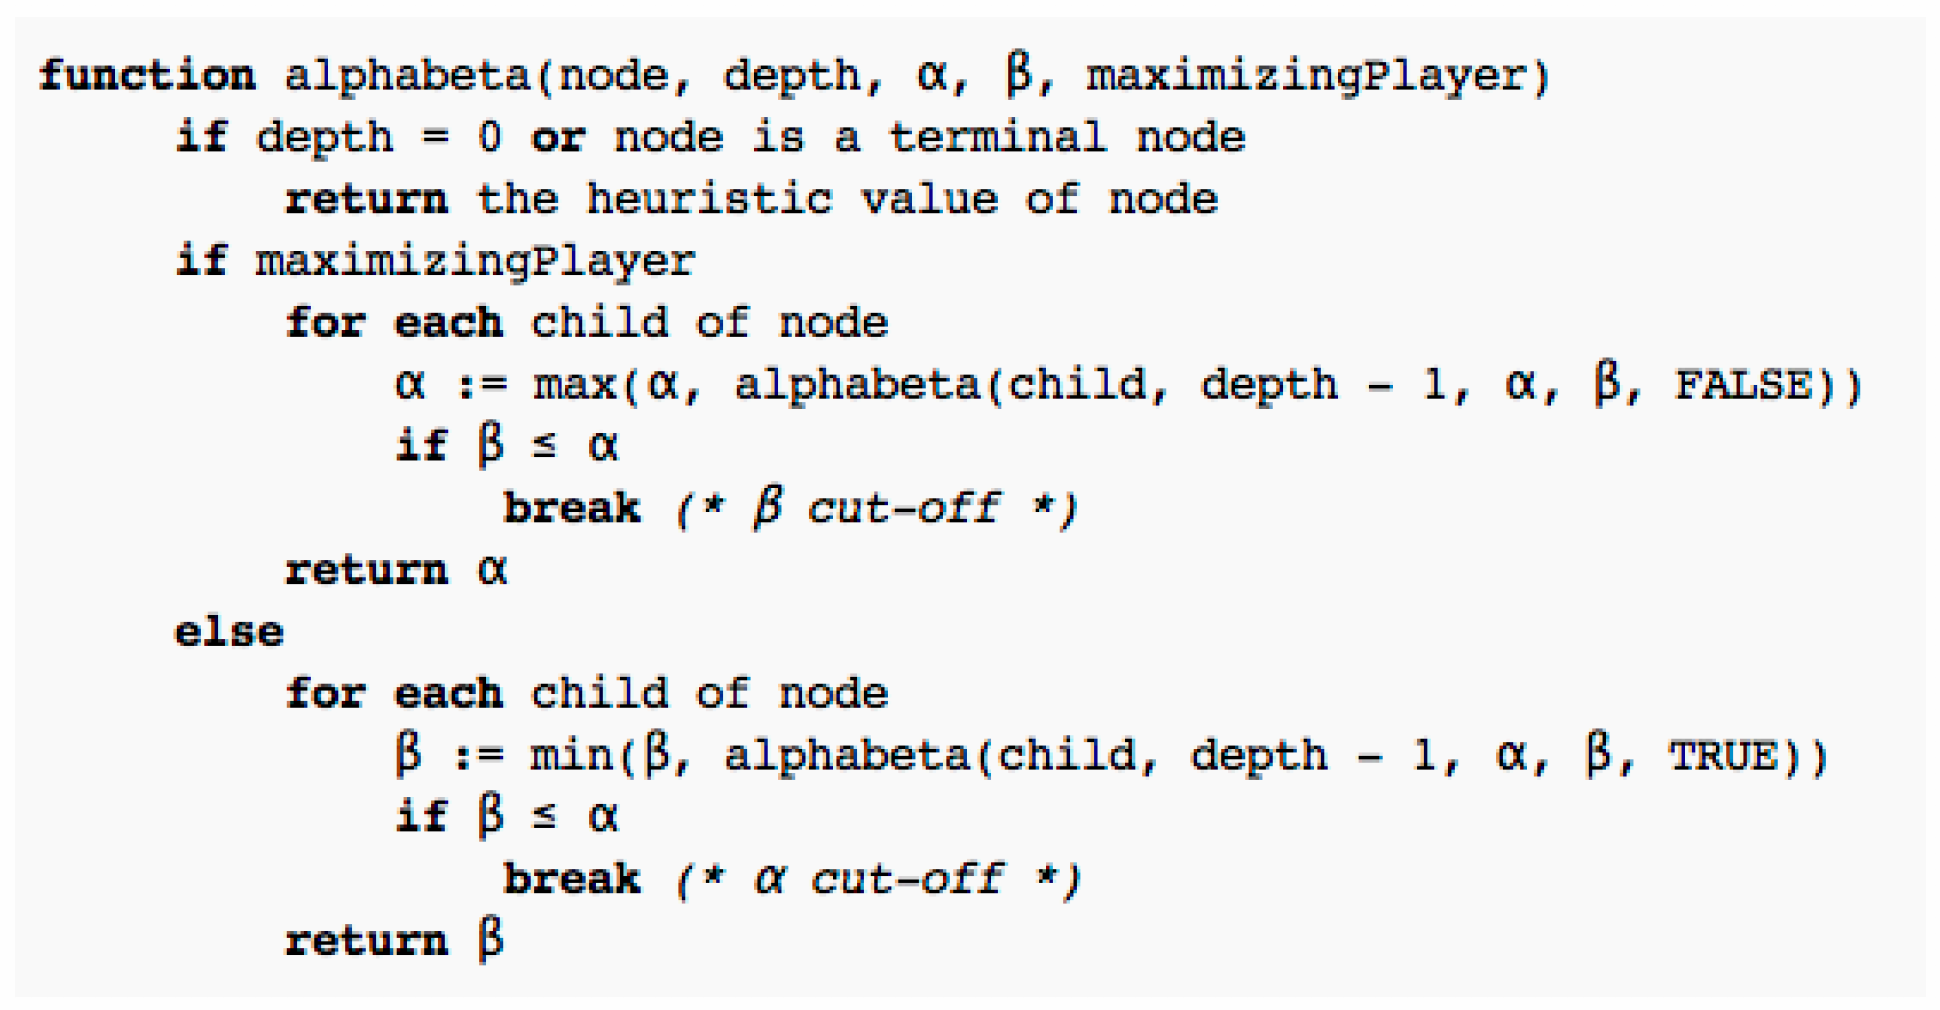
\includegraphics[width=0.5\textwidth]{img/01_sequential_games/alphabeta_pseudocode.png}
			\caption{Pseudocode eines Minimax mit limitierter Tiefe mithilfe von Alpha-Beta Pruning}
			\label{fig:01_seq_alphabeta_pseudocode}
		\end{figure}
	
		\paragraph{Speed-Up of Alpha-Beta Pruning}
		
		\begin{itemize}
			\item In einem Spielbaum mit Tiefe $m$ mit $b$ möglichen Aktionen bei jedem Knoten ist die Zeitkomplexität des Minimax O($b^{m}$) bzw.. es gibt b$^{m}$ Blattknoten
			\item Im Idealfall benötigt Alphe-Beta Pruning nur O($b^{m/2}$) = O($(\sqrt{b})^{m}$). 
			Dies korrespondiert zu einer Reduzierung des Branching-Faktors von $b$ zu $\sqrt{b}$, bspw. bei Schach bedeutet dies 6 mögliche Aktionen bei jedem Knoten (anstelle von 35)
			\item Um diesen maximalen Speed-Up zu erreichen, müssen die verschiedenen States in gescheiter Anordnung erforscht werden, was jedoch problemspezifisch ist.
		\end{itemize}
	
	\section{Monte Carlo Tree Search}
	
		\subsection{Random Walks}
		
		\begin{itemize}
			\item Suchräume sind meist zu gross für eine vollständige Suche
			\item Minimax soll bei einer bestimmten Baum-Tiefe stoppen und raten (mit Heuristik)
			\item Monte Carlo Tree Search ist ein anderes Vorgehen: \\
			\textit{Monte Carlo Tree Search führt Random Walks durch, um möglichst viel des Suchbaums in einem vorbestimmten Zeitraum abzusuchen.
			Danach wird der vielversprechendste Zug gespielt.}
		\end{itemize}
	
		\newpage
	
		\subsection{The 4 Phases in Monte Carlo Tree Search}
		
		\begin{enumerate}
			\item \textbf{Selection}
				\begin{itemize}
					\item Starte beim Wurzelknoten \texttt{R} und wähle fortlaufend Kinderknoten
					\item Stoppe, wenn du einen Knoten erreichst, der noch nicht komplett erweitert/erforscht wurde
					\item Benötigt ein Kriterum für die Auswahl der Kinderknoten, sogennante \textit{tree policy}
				\end{itemize}
			\item \textbf{Expansion}
				\begin{itemize}
					\item Wenn das Zeitlimit \texttt{L} das Spiel beendet, gib die Payoffs zurück
					\item Sonst, wähle eine unerforschte Aktion und kreiere einen Knoten \texttt{C} für diese
				\end{itemize}
			\item \textbf{Simulation}
				\begin{itemize}
					\item Simuliere ein Weiterspielen von Knoten \texttt{C} aus, mithilfe einer \textit{default policy}
					\item Im simpelsten Fall, spiele einfach bis zu irgendeinem Ende mit zufälligen Zügen
				\end{itemize}
			\item \textbf{Backpropagation}
				\begin{itemize}
					\item Aktualisiere die gespeicherten Informationen in jedem Knoten von \texttt{C} zurück bis zu \texttt{R}
					\item MCTS erwartet einen Payoff in [0,1]
				\end{itemize}
		\end{enumerate}
	
		\subsection{MCTS for Tic-Tac-Toe}
		
		\begin{figure}[htb!]
			\centering
			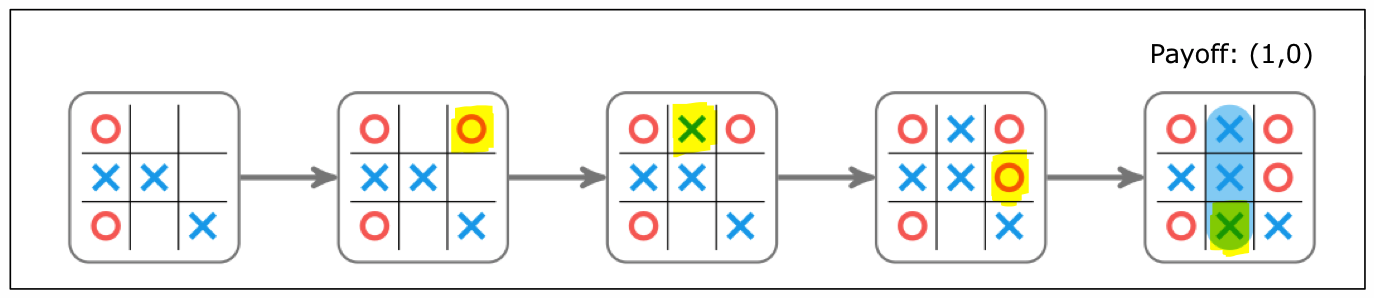
\includegraphics[width=0.6\textwidth]{img/02_mcts/random_ttt.png}
			\caption{Zufälliger Durchlauf eines Runde Tic-Tac-Toe}
			\label{fig:02_mcts_random_tictactoe}
		\end{figure}
	
		\begin{itemize}
			\item Es gibt Punkte für einen Gewinn (1), unenentschieden (0.5) und Verlust (0)
			\item MCTS ist nicht limitiert auf zero-sum Spiele
			\item Payoffs werden durch Vektoren repräsentiert
			\item Die Simulation endet mit einem Gewinn für Spieler X mit Payoff +1 $\rightarrow$ Payoff-Vektor (1,0) \\
			(Spieler Y hat in dieser Simulation also einen Payoff von 0)
		\end{itemize}
	
		\begin{figure}[htb!]
			\centering
			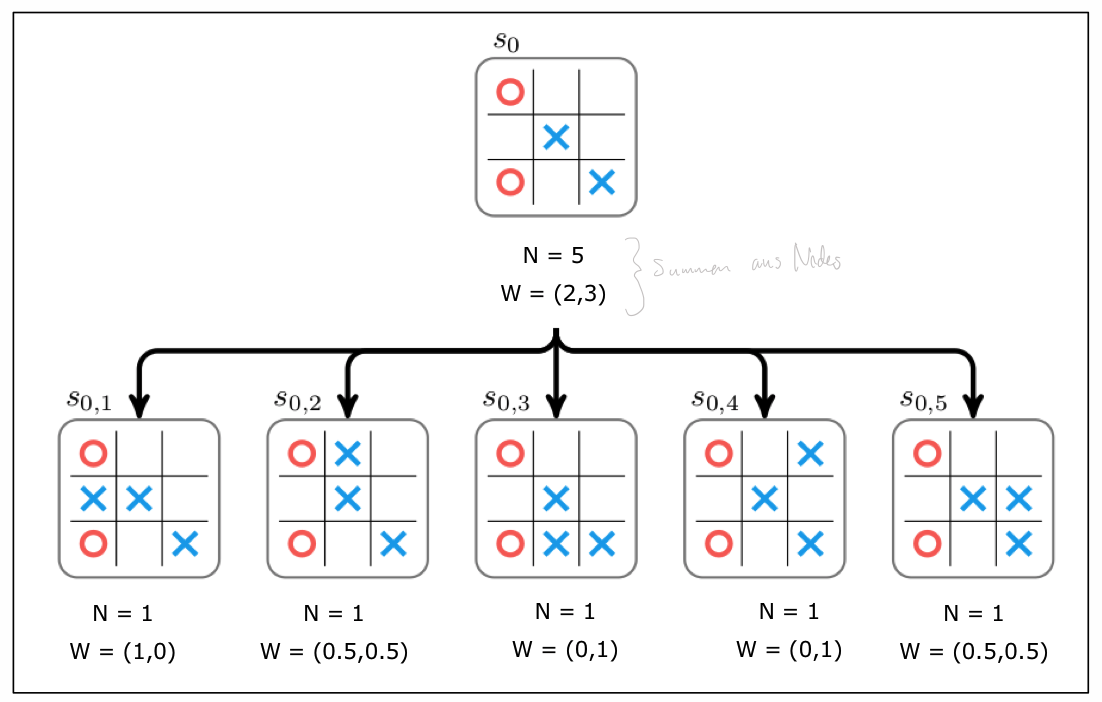
\includegraphics[width=0.6\textwidth]{img/02_mcts/ttt_payoffs.png}
			\caption{übersicht der Simulationen eines Tic-Tac-Toe Spiels}
			\label{fig:02_mcts_ttt_payoffs}
		\end{figure}
	
		\begin{itemize}
			\item \texttt{N} speichert die Anzahl Simulationen, die vom Knoten $s_{0}$ aus gestartet wurden
			\item \texttt{W} sind die akkumulierten Payoff-Vektoren (eine Komponente für jeden Spieler)
			\item Backpropagation kalkuliert lediglich die Summe von \texttt{N}$^{*}$ und \texttt{W}
			\item \textbf{Wichtig}: Ist der Wurzelknoten ebenfalls auch ein Kindesknoten, muss sein Payoff nach oben ebenfalls hinzugerechnet werden 
		\end{itemize}
	
		\newpage
	
		\subsection{Selection Policy: Which Node to Choose}
		
		\begin{figure}[htb!]
			\centering
			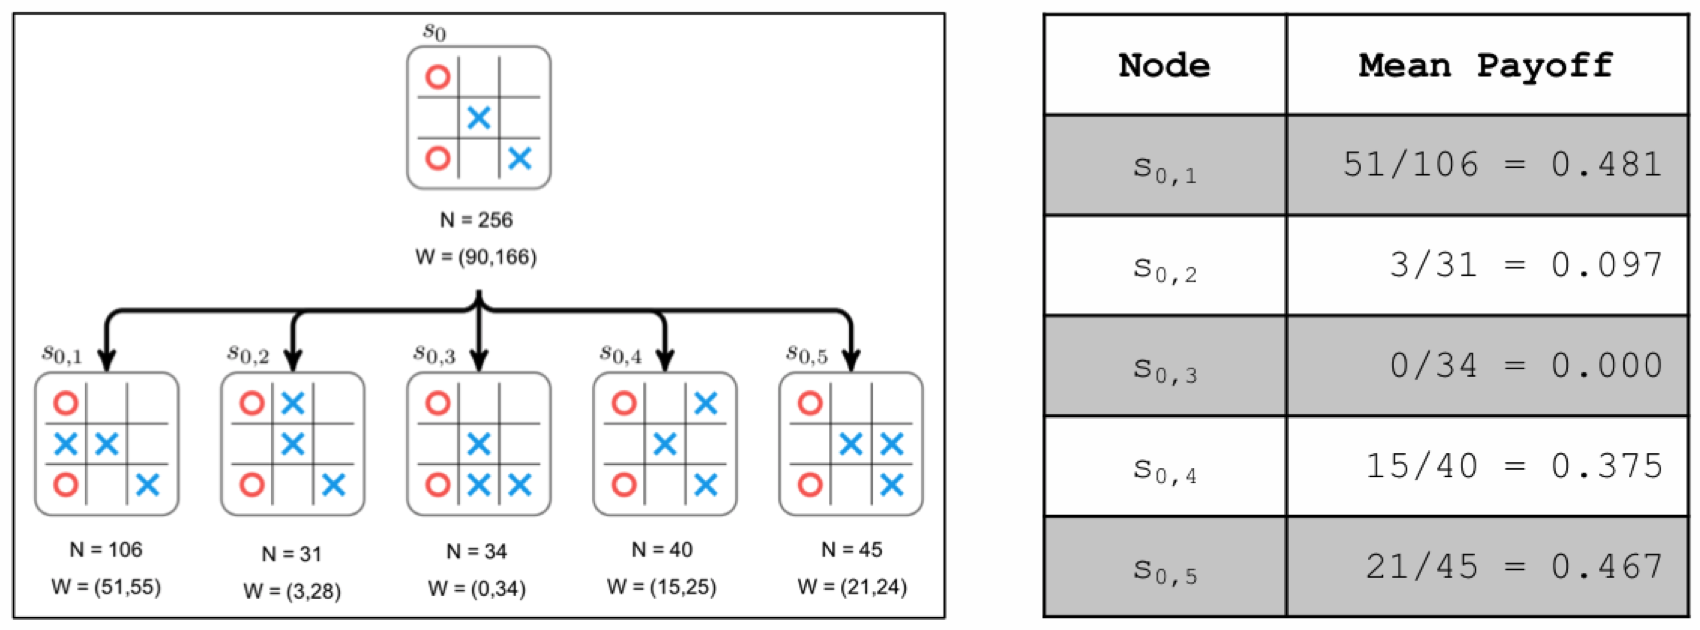
\includegraphics[width=0.6\textwidth]{img/02_mcts/selection_policy.png}
			\caption{Durchschnittliche Payoffs der durchlaufenen Simulationen mit MCTS}
			\label{fig:02_mcts_selection_policy}
		\end{figure}
		
		\begin{itemize}
			\item \textbf{Exploitation} \\
			Knoten $s_{0,1}$ hat den höchsten durchschnittlichen Payoff bzw. basierend auf aktuell verfügbaren Informationen, maximiert dieser Knoten meinen erwarteten Gewinn
			\item \textbf{Exploration} \\
			Knoten $s_{0,4}$ wurde nur 40 mal probiert, wie kann ich sicher sein dass der Score tiefer bleibt als bei $s_{0,1}$, auch wenn ich jetzt noch 66 mal spielen würde?
		\end{itemize}
	
		\subsection{Example of Multi-Armed Bandits}
		
		\begin{itemize}
			\item Es gibt eine Reihe an Slotmaschinen mit verschiedenen (unbekannten) Auszahlungswahrscheinlichkeiten und -mengen
			\item Man hat 1000 Münzen und möchte den erwarteten Gewinn erhöhen
			\item Idealerweise würde man immer an der Maschine mit dem grössten erwarteten Gewinn spielen
			\item Unglücklicherweise weiss man jedoch nicht, welche Maschine dafür am besten ist
			\item Es ist keine Person da, welcher man zuschauen und mehr über die Maschinen erfahren kann
		\end{itemize}
		\vspace{1em}
		Wie wählt man nun die beste Strategie in dieser Situation?
	
		\subsection{UCB1: Upper Confidence Bound}
		
		\begin{itemize}
			\item Am besten Exploration und Exploitation ausbalancieren
				\begin{itemize}
					\item \textbf{Exploration}: Spiele alle Maschinen um möglichst viele Informationen zu sammeln
					\item \textbf{Exploitation}: Spiele die beobachtet beste Maschine um den erwarteten Gewinn zu maximieren
				\end{itemize}
			\item UCB1 bietet die beste Balance zwischen Exploration und Exploitation, es gibt quasi ein statistisches Vertrauensintervall für jede Maschine aus
				\begin{itemize}
					\item Parameter $c \geq 0$ kontrolliert den Trade-Off zwischen Exploitation (tiefes $c$) und Exploration (hohes $c$)
				\end{itemize}
		\end{itemize}
	
		$$U_{i} = \frac{W_{i}}{N_{i}} + c \sqrt{\frac{\ln N_{p}}{N_{i}}}$$
		
		\vspace{1em}
		\begin{description}
			\item[$\frac{W_{i}}{N_{i}}$] \textbf{Exploitation}, der durchsch. Gewinn für Maschine $i$ ($\frac{Gewinne}{Versüche}$)
			\item
			\item[$\sqrt{\frac{\ln N_{p}}{N_{i}}}$] \textbf{Exploration}
				\begin{description}
					\item[$N_{p}$] Wie oft haben wir insgesamt gespielt (wie viele Münzen wurden verbraucht)
					\item[$N_{i}$] Wie oft wurde Maschine $i$ ausprobiert
				\end{description}
		\end{description}
		
		\newpage
		
		\paragraph{How to play with UCB1}
		Für jede der 1000 Münzen...
		\begin{itemize}
			\item Kalkuliere das UCB1 ($U_{i}$) von jeder Maschine $i$
			\item Spiele an der Maschine mit dem höchsten Upper Bound ($U_{i}$)
			\item Wähle entweder zufällig oder in nummerischer Ordnung
		\end{itemize}
		
		
		
	
	\section{Information Sets}
	
	
	
	\section{Supervised Machine Learning}
	
	
	
	\section{Neuronal Networks}
	
	
	
	\section{Deep Neuronal Networks}
	
	
	
	\section{Convolutional Neuronal Networks}
	
	
\end{document}
